\documentclass{article}
\usepackage[ruled,vlined]{algorithm2e}
\usepackage{latexsym}
\usepackage{amssymb}
\usepackage{amsmath}
\usepackage{amsthm}
\usepackage{epsfig} 
\usepackage{fullpage}
\usepackage{url}
\usepackage{enumerate}
\usepackage{xspace}
\usepackage{marvosym}
\usepackage{listings}


\begin{document}
\begin{titlepage}
\center
\textsc{\LARGE{Different clasp configurations in D-FLAT}}\\[1.5cm]
\textsc{\large{Project Report}}\\[1cm]
\textsc{\large{database and artificial intelligence group}}\\
\textsc{\large{Faculty of Informatics, TU Vienna}}\\[1.5cm]
\begin{minipage}{0.4\textwidth}
	\begin{flushleft} \large
		\emph{Author:}\\
		Dino \textsc{Rossegger} % Your name
	\end{flushleft}
\end{minipage}
\begin{minipage}{0.4\textwidth}
	\begin{flushright} \large
		\emph{Supervisors:} \\
	\end{flushright}
\end{minipage}\\[4cm]
{\large \today}\\[2cm]
\end{titlepage}

\section{Introduction}
The D-FLAT project, developed by the DBAI group of TU Vienna, makes use of problem structure to solve reasoning problems with the help of Answer Set Programming.
It uses \emph{tree decompositions} to decompose the problem into smaller subproblems and then uses traditional ASP solvers to solve the subproblems, combining the solutions until a solution for the whole problem is obtained.

D-FLAT uses clasp as ASP solver. clasp is a powerful solver offering vast possibilities to optimize its performance. While the default configuration is robust for most problems, it is the case that for some problems, different configurations perform better. Identifying those problems by hand is tedious and most of the time not desirable, therefore claspfolio was developed whichuses algorithm selection techniques to automatically select promising configurations. This resulted in a huge performance gain, allowing claspfolio to outperform traditional ASP solvers.

The goal of the project was to apply algorithm selection techniques for clasp as used in claspfolio to see how this affects the performance of D-FLAT. Since D-FLAT only uses clasp to solve subproblems it was not clear how algorithm selection techniques affect its performance.
\section{Design}
The first idea was to perform algorithm selection at every \inline$clasp$ call made by \mbox{D-FLAT}. In theory this approach achieves the most performance gain since the best configuration is used for every call but since \inline$clasp$ is called mostly on small subproblems which are relatively easy to solve, the overhead generated by the algorithm selection would likely be too high such that the gains in performance cannot compensate the cost of the selection process.

Another approach is to only analyse the main problem by looking at features of the ungrounded instance and select the best configuration based on this features for all \inline$clasp$ calls. The disadvantage of this approach is that a good configuration for the problem might not be a good configuration for its subproblems but since most of the subproblems are easy to solve and big subproblems have most likely a similar structure as the problem, it might still be feasible.

The first approach needs careful implementation to work efficiently and the use of existing technologies is harder than in the second approach. Since it was also not known if algorithm selection techniques benefit \mbox{D-FLAT} at all, it was more feasible to use the second approach to investigate if the tuning of \inline$clasp$ using algorithm selection has an impact on the performance of \mbox{D-FLAT}.


\section{Implementation}
\label{sec:impl}
\subsection{System Architecture}
To help D-FLAT profit from machine learning techniques an architecture based on the architecture proposed in ~\cite{DBLP:conf/lpnmr/GebserKKSSZ11} was used. The architecture is shown in Figure~\ref{impl:sysarch}. First instance features are extracted, then a prediction which solver configuration will be the best is made using machine learning algorithms and finally D-FLAT is launched with the predicted configuration.
\begin{figure}[h]
	\center
	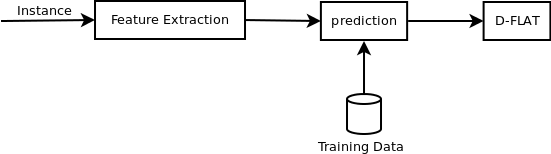
\includegraphics[scale=0.6]{figures/sysarch.png}
	\caption{System Architecture of D-FLAT with Learning\label{impl:sysarch}}
\end{figure}
A python script was implemented to handle the control flow such that the user only has to supply the instance and learning database. Furthermore some modifications to D-FLAT were made to allow the configuration of the solver.

\subsection{Modifications to D-FLAT}
To the default configuration four different clasp configurations were added using \lstinline$clasp_fascade$ of its library. The three configurations \emph{jumpy},\emph{frumpy},\emph{crafty} aim to copy the portfolios provided by clasp, while \emph{nopre} instructs clasp to skip any preprocessing and start solving directly. These configurations where added to the \lstinline$Asp$ class in D-FLAT. Users can set the desired portfolio by using the \lstinline$--portfolio$ flag followed by the name of the portfolio in the command line arguments.

Another new flag \lstinline$--ext-feat$ instructs D-FLAT to stop processing after decomposing the instance and print out its decomposition width in machine readable format. This flag is used for feature extraction. Additional feature extractors can be implemented by writing subclasses of \lstinline$FeatureExtractor$ and adding corresponding instances to the list \lstinline$felist$ in the $Algorithm$ class.
\subsection{Feature Extraction}
Apart from features extractable from D-FLAT also features from other sources are used. Features of the encoding are extracted using \lstinline$gringos$ \lstinline$--gstats$ flag and some features are extracted directly from the instance file. A complete list of available features can be seen in Table~\ref{tbl:feat}.

\begin{table}
	\center
	\begin{tabular}{|l|l|l|}
		\hline
		Name & Description & Origin \\
		\hline
		\lstinline$gcomponents$ & number of components\footnote{$function symbols+ predicate symbols$} & gringo\\ %TODO Fix footnote
		\lstinline$gnontrivial$ & number of nontrivial components & gringo\\
		\lstinline$gpredicates$ & number of predicates & gringo \\
		\lstinline$gconstraints$ & number of constraints & gringo\\
		\lstinline$nbredgefacts$ & number of edge facts & instance file\\
		\lstinline$nbredgepred$ & number of edge predicates & user \\
		\lstinline$defjoin$ & $1$ if D-FLATs default join was used, $0$ otherwise & user\\
		\lstinline$normalization$ & the normalization used (non, semi, normalized) & user\\
		\lstinline$heuristic$ & the heuristic used to create the tree decomposition & user\\
		\lstinline$dw$ & the decomposition width of the tree decomposition & D-FLAT\\
		\hline
	\end{tabular}
	\caption{Features of the datasets}
	\label{tbl:feat}
\end{table}
The feature extraction is handled by the python script \emph{Learner}.

\subsection{Learner}
The program \emph{Learner} has been developed to handle all machine learning related tasks. \emph{Learner} supports $3$ subcommands \lstinline$learn, genmod$ and \lstinline$solve$. 
\lstinline$learn$ instructs \lstinline$learner$ to build the learning base or training set as it is often called and save it in $csv$ style. 
\lstinline$genmod$ generates a Support Vector Machine model based on the training set and \lstinline$solve$ is used to actually solve instances. Detailed information on the different subtools is given in the following subsections.

Basic configuration of \emph{Learner} is done with the \lstinline$config.xml$ file in its main directory. For further detail on the configuration look at the example provided in the distribution. Table~\ref{tbl:req} shows \emph{Learners} system requirements.

\begin{table}[h]
	\center
	\begin{tabular}{ll}
		Requirement & Version\\
		python & $\geq2.7$\\
		gringo & $\geq3.0$\\
		scikit-learn & $\geq0.10$\\
		D-FLAT learn & $\geq0.01$
	\end{tabular}
	\caption{Learner system requirements \label{tbl:req}}
\end{table}

\paragraph{\lstinline$learn$}
It is encouraged to use \lstinline$learn$ to build training sets. For every instance provided in the \lstinline$config.xml$ \emph{Learner} first extracts the features of the instance. Then it calls D-FLAT with each portfolio and measures the runtime using \lstinline$time$~\cite{www:time}.
Using the flags \lstinline$--mtime$ and \lstinline$--reslimit$ the execution time and resource usage can be limited for the processes. If one of these limits is reached \emph{Learner} kills the instance and reports $-100$ as runtime, telling that this instance was not solvable with the respective portfolio. It then writes all features and runtimes to a file, the destination of this file can be specified using \lstinline$--learningbase$, as default \lstinline$learningbase.csv$ is used. The learning base can be used to build the machine learning model using \lstinline$genmod$.

\paragraph{\lstinline$genmod$}
Invoking this command tells \emph{Learner} to build a model of the learningbase specified by the flag \lstinline$--learningbase$. Support Vector Machines as implemented by scikit-learn~\cite{www:scikit} are used as classifier. Numerical features are scaled such that they have $0$ mean and unit variance using scikit-learns \lstinline$StandardScaler$. 
Nominal features are encoded using $1-of-K$ encoding, i.e. for $K$ different values each value is represented by a binary vector of $K$ length where exactly $1$ bit has the value $1$ and all others $0$.
After this preprocessing steps the model is fitted to the learningbase and saved to \lstinline$default.mod$, to choose a different location \lstinline$--model$ can be used.

\paragraph{\lstinline$solve$}
is used to solve instances with the best portfolio predicted by the model generated by \lstinline$genmod$. The model is specified using \lstinline$--model$, \lstinline$-e$ is used to specify the edge predicates, other arguments for D-FLAT can be specified as string using \lstinline$--arg$.
\lstinline$Learner$ then predicts the best portfolio based on the specified model and launches D-FLAT with it. Any output generated by D-FLAT is shown in the command line.




\section{Benchmarks}\label{sec:benchmarks}
$20$ instances of SAT and $81$ instances of Dominating Set have been benchmarked using their respective \mbox{D-FLAT} problem encodings. SAT instances have been tested with the available decomposition normalization types none, semi and weak normalization. Semi and weak normalizations have been run once using \mbox{D-FLAT}'s default-join and once using the join rules supplied in the encoding. 
Since the encoding did not support default-join, Dominating Set instances have been tested only with semi and weak normalization without default-join. This resulted in $266$ instances.

The benchmarks have been carried out on a machine with $4$ AMD Opteron $6308$ processors each having $3500$ $MHz$ and $192$ $GB$ of RAM, however only $1$ core was used.

At first the features of each instance were extracted, then \mbox{D-FLAT} was called for each of the five portfolios using a fixed seed for the decomposition heuristics to ensure integrity of the results.
Execution was handled by the \inline$learn$ subcommand of \inline$Learner$ using Pythons subprocess module~\cite{www:subprocess}, the resource module~\cite{www:resource} was used to restrict the maximum memory an instance could use to $24$ $GB$. To get exact runtime results GNU time~\cite{www:time} was used. If a process did not finish after $40$ minutes it was killed and its runtime set to $-100$. Real, user and system time as reported by GNU time were logged together with the exit code and features of the instance and then saved in \inline$csv$ format.

\subsection{Instance details}
The Dominating Set instances were taken from an earlier experiment. Hence the runtime of the instances could be estimated by their runtime in this experiment and instances having too high runtime ($>10$ minutes) were filtered out. Therefore all of these instances finished in time without exceeding the resource limit.

The SAT instances were generated using the generator supplied in the \mbox{D-FLAT} package. Because of the generators randomness the instances were varied, containing unsolvable instances as well as very easy instances solvable in a few milliseconds.

\subsection{Analysis}
Out of the $100$ SAT instances $19$ had to be terminated because they ran out of time. The distribution of runtimes can be seen in Figure~\ref{fig:runtime}.

\begin{figure}[h]
	\center
	
\includegraphics[scale=\figscale]{figures/runtime.png}
	\caption{Distribution of the runtime of the benchmarks\label{fig:runtime}}
\end{figure}

The most improved runtime compared to the unconfigured solver, was achieved in a SAT instance where the portfolio \inline$crafty$ was $2.29$ times faster. On average the unconfigured solver was $7.4\%$ slower than the best portfolio, having a median of $3.9\%$. A summary of the characteristics is given in Table~\ref{tbl:charcmp}.

\begin{table}[h]
	\center
	\begin{tabular}{c|c|c|c|c|c}
		Min. & $1^{st}$ Quartile & Median & Mean & $3^{rd}$ Quartile & Max. \\
		\hline
		$1.000$&$1.005$&$1.039$&$1.074$&$1.082$ &$2.290$
	\end{tabular}
	\caption{Characteristics of the unconfigured solver compared to the best configuration\label{tbl:charcmp}}
\end{table}

\begin{figure}[h]
	\center
	
\includegraphics[scale=\figscale]{figures/relativePerformance.png}
	\caption{Performance of \inline$clasp$ without portfolio in comparison to the fastest portfolio\label{fig:perf}}
\end{figure}

The performance of the standard configuration of \inline$clasp$ in comparison to other portfolios can be seen in Figure~\ref{fig:perf}. The figures are obtained by dividing the runtime of the default configuration by the runtime of the fastest portfolio.
Interestingly for Dominating Set other portfolios were clearly better the majority of times while for SAT a difference between the standard configuration and any portfolio seems marginal except for some extreme outliers.

\section{Machine Learning Tests}
\label{sec:ml}
Classification experiments where carried out to test if the data retrieved in the benchmarks lends itself to classification. The experiments where carried out using WEKA~\cite{WEKA}, as classifier support vectore machines where used through the \lstinline$libsvm$ package available for all major operating systems. The classifier was tested using $10$-fold cross validation on the \emph{Dominating Set} and \emph{SAT} dataset obtained from the benchmarks seperatly as well as both datasets joined. The data was labeled with numbers $0-6$ for the fastest portfolio according to the \emph{user} time from the benchmarks.
The labels together with its portfolio can be seen in Table~\ref{tbl:mlLabel}. The experiments have been performed on the data with and without the label $6$, \emph{eq} which says that the runtimes were equal for all instances. For the experiments without the \emph{eq} label the instances with equal runtimes have been labelled $5$.
\begin{table}[h]
	\center
	\begin{tabular}{|r|l|}
		\hline
		Label & Portfolio\\
		\hline
		0 & not solved\footnote{The instance was not solved by any portfolio in the given time limit} \\
		1 & jumpy\\
		2 & frumpy\\
		3 & crafty\\
		4 & none \\
		5 & nopre\\
		6 & eq\\
		\hline
	\end{tabular}
	\caption{Labels assigned to the corresponding portfolios}
	\label{tbl:mlLabel}
\end{table}


\par $11$ features were used in the classification experiments. The features and their origin can be seen in Table~\ref{tbl:mlFeat}, details about the extraction can be found in Section~\ref{sec:impl}. Features tagged with \emph{user} are features usually supplied by the user when executing D-FLAT, the number of edge facts is counted in the input file and features tagged $gringo$ are features of the non-ground instance. They are also independent of the instance and therefore have the same value for all instances of an encoding. 

Before the models were built, feature selection techniques were applied to get a feel which features effect the model the most.

\begin{table}
	\center
	\begin{tabular}{|l|l|l|}
		\hline
		Name & Description & Origin \\
		\hline
		\lstinline$gcomponents$ & number of components\footnote{$function symbols+ predicate symbols$} & gringo\\
		\lstinline$gnontrivial$ & number of nontrivial components & gringo\\
		\lstinline$gpredicates$ & number of predicates & gringo \\
		\lstinline$gconstraints$ & number of constraints & gringo\\
		\lstinline$nbredgefacts$ & number of edge facts & instance file\\
		\lstinline$nbredgepred$ & number of edge predicates & user \\
		\lstinline$defjoin$ & $1$ if D-FLATs default join was used, $0$ otherwise & user\\
		\lstinline$normalization$ & the normalization used (non, semi, normalized) & user\\
		\lstinline$heuristic$ & the heuristic used to create the tree decomposition & user\\
		\lstinline$dw$ & the decomposition width of the tree decomposition & D-FLAT\\
		\hline
	\end{tabular}
	\caption{Features of the datasets}
	\label{tbl:mlFeat}
\end{table}

\subsection{Experiments without \emph{eq}}
\subsubsection{Dominating Set}
The distribution of the labels can be seen in Figure~\ref{fig:dsLabelsE1}. There are no $term$ labels in this dataset since it was used prior for benchmarks and instances with runtime over the time limit where not executed again.
\begin{figure}[h]
	\center
	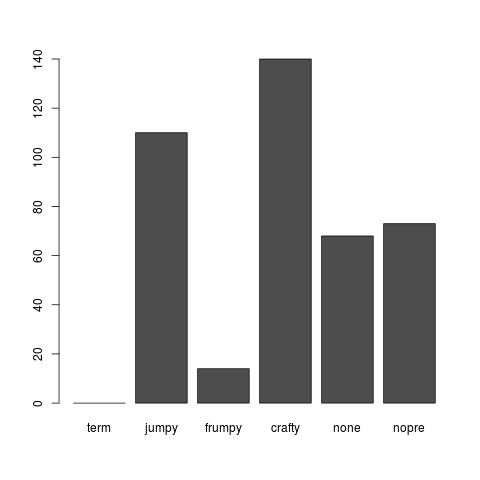
\includegraphics[scale=0.4]{figures/domsetLabelsE1.png}
	\caption{Distribution of labels of Dominating Set\label{fig:dsLabelsE1}}
\end{figure}
\par Three feature selection methods were used on the dataset all yielding the same result that the features \lstinline$defjoin$ and \lstinline$normalization$ are the only features impacting the model significantly in both experiments. The model was therefore built on those two features as well as on all features.

\par The model on all features had $Precision$\footnote{$Precision=\frac{tp}{tp+fp}$}$=0.39$ and $Recall$\footnote{$Recall=\frac{tp}{tp+fn}$}$=0.41$, yielding $F_1-score$\footnote{$F_1=2*\frac{precision*recall}{precision+recall}$}$=0.36$.
Using only the two aforementioned features resulted in a slightly better model having $Precision=0.4$ and $Recall=0.44$, yielding $F_1-score=0.41$. The confusion matrix for both models can be seen in Table~\ref{tbl:dsCME1}. 
\begin{table}[h]
\center
	\begin{tabular}{|c|ccccc|ccccc|}
		\hline
		\multicolumn{6}{|c|}{All Attributes} &\multicolumn{5}{|c|}{normalization, defjoin}\\
		\hline &$1$&$2$&$3$&$4$&$5$&$1$&$2$&$3$&$4$&$5$\\
		 \hline$1$&$23$&$0$&$77$ &$8$ &$1$&$62$&$0$&$42$&$2$&$3$\\
		 $2$&$3$ &$0$&$10$ &$1$ &$0$&$3$ &$0$&$5$ &$1$&$5$\\
		 $3$&$26$&$0$&$106$&$5$ &$3$&$63$&$0$&$64$&$6$&$7$\\
		 $4$&$9$ &$0$&$42$ &$12$&$5$&$1$ &$0$&$48$&$3$&$16$\\
		 $5$&$14$&$0$&$27$ &$30$&$3$&$2$ &$0$&$21$&$1$&$50$\\
		 \hline
	\end{tabular}
	\caption{Confusion Matrix for Dominating Set}
	\label{tbl:dsCME1}
\end{table}
\par The model using all features overclassifies instances as $3$ (\emph{crafty}), resulting in a high recall of $77.5$ of this label but bad recall for all other labels. The precision however remains fairly balanced throughout the labels. It is interesting to see that both classifiers were not able to label an instance of $2$ (\emph{frumpy}) correctly since there are only very few instances labeled $2$ in the dataset. The classifier on only \lstinline$normalization$ and \lstinline$defjoin$ still leans to overclassifying instances as $3$ but not to the same extent as the model working on all features.
Therefore it has better precision of $0.62$ and is overall the slightly better classifier. This also shows when looking at the correctly classfied instances. The model built on all features classified $41\%$ of the instances correctly, while the model built on only $normalization$ and $defjoin$ classified $45\%$ correctly.

\subsubsection{SAT}
The distribution of the labels of the instances can be seen in Figure~\ref{fig:satLabelsE1}. This dataset contains instances which could not be solved in the specified maximum time in the benchmark, even the majority of the instances belongs to that class. 

\begin{figure}[h]
	\center
	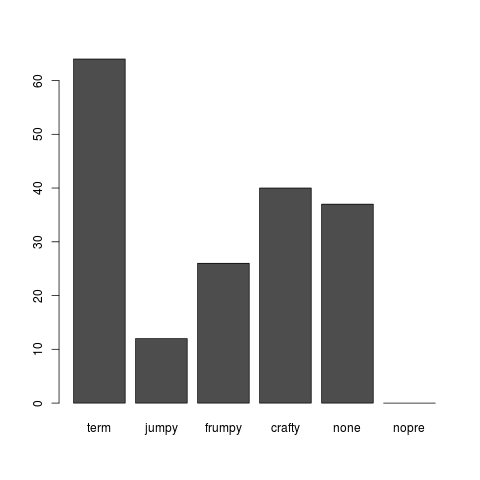
\includegraphics[scale=0.4]{figures/satLabels.png}
	\caption{Labels of SAT\label{fig:satLabelsE1}}
\end{figure}

\par Again feature selection methods were used to determine the features with the most impact on the result. Interestingly the heuristics determined $dw$ and $nbredgefacts$ to have big impact, $normalization$ and $defjoin$ to have a little bit of impact and the other features to have very little to no impact on the prediction quality. Therefore models where built using these four features, all features  and only $dw$,$nbredgefacts$.

The model built on all features has $precision=0.32$ and $recall=0.42$, yielding $F_1=0.35$ while the model built on $nomalization$, $dw$, $nbredgefacts$ and $defjoin$ has $precision=0.31$ and $recall=0.41$, yielding $F_1 =0.35$. The classifier built of only $dw$ and $nbredgefacts$ has $precision=0.32$ and recall $F_1=0.42$. According to the $F_1$ score the model on all features and the model built on only $dw$ and $nbredgefacts$ perform equally, while the model built on the four features predicted best by the feature selection heuristics performs sligthly worse. Looking at the correctly classified instances this effect can be seen too. The models on all features and on $dw$ and $nbredgefacts$ classified $42$ ($42\%$) correctly, while the model on four features classified $41$ ($41\%$) instances correctly. The confusion matrix for the models can be seen in Table~\ref{tbl:satCME1}.

\begin{table}[h]
	\center
	\begin{tabular}{|c|cccccc|cccccc|cccccc|}
		\hline\multicolumn{7}{|c|}{All Attributes} &\multicolumn{6}{|c|}{$4$ attributes}&\multicolumn{6}{|c|}{dw, nbredgefacts}\\
		\hline &$0$&$1$&$2$&$3$&$4$&$5$&$0$&$1$&$2$&$3$&$4$&$5$&$0$&$1$&$2$&$3$&$4$&$5$\\
		\hline $0$ & $4$ & $0$ & $0$ & $2$ & $1$ & $12$& $4$ & $0$ & $0$ & $2$ & $2$ & $11$& $4$ & $0$ & $0$ & $3$ & $2$ & $10$\\
					 $1$ & $1$ & $0$ & $0$ & $0$ & $0$ & $3$ & $1$ & $0$ & $0$ & $0$ & $0$ & $3$ & $1$ & $0$ & $0$ & $0$ & $0$ & $3$\\
					 $2$ & $1$ & $0$ & $0$ & $0$ & $1$ & $2$ & $1$ & $0$ & $0$ & $0$ & $1$ & $2$ & $1$ & $0$ & $0$ & $0$ & $1$ & $2$\\
					 $3$ & $3$ & $0$ & $0$ & $0$ & $2$ & $5$ & $3$ & $0$ & $0$ & $0$ & $2$ & $5$ & $3$ & $0$ & $0$ & $0$ & $2$ & $5$\\
					 $4$ & $4$ & $0$ & $0$ & $0$ & $3$ & $12$& $4$ & $0$ & $0$ & $0$ & $3$ & $12$& $4$ & $0$ & $0$ & $1$ & $3$ & $11$\\
					 $5$ & $4$ & $0$ & $0$ & $0$ & $5$ & $35$& $5$ & $0$ & $0$ & $0$ & $5$ & $34$& $5$ & $0$ & $0$ & $0$ & $4$ & $35$\\
		\hline
	\end{tabular}
	\caption{Confusion Matrix for SAT}
	\label{tbl:satCME1}
\end{table}
\subsubsection{All Instances}
The experiments in this section are the most meaningful since they work with the data from both benchmarks. The input data was obtained by combining the data from both benchmarks.

Again feature selection heuristics were used on the dataset, selecting a subset of $4$ features, $gcomponents$, $gnontrivial$, $nbredgefacts$ and $dw$ as the most impactful features. In contrast to the other experiments all features but $heuristic$ had some impact on the result. Therefore models were built on the subset as well as on all features.

The model built on all features has $precision=0.38$ and $recall=0.42$, yielding $F_1=0.38$, while the model built on the subset performed worse, having $precision=0.3$ and $recall=0.35$, yielding $F_1=0.31$. The model build on all features classified $42\%$ of the instances correctly, while the model built on the subset classified $35\%$ correctly. This strengthens the observation made during feature selection that all features but $heuristic$ impact the result. Another experiment was made using all features but $heuristic$, producing exactly the same results as the experiment on all features, strengthening the observation even further. The confusion matrix of both models can be seen in Table~\ref{tbl:cmbCM}.

\begin{table}[h]
	\center
	\begin{tabular}{|c|cccccc|cccccc|}
		\hline\multicolumn{7}{|c|}{All Attributes} &\multicolumn{6}{|c|}{$4$ attrib}\\
		\hline &$0$&$1$&$2$&$3$&$4$&$5$&$0$&$1$&$2$&$3$&$4$&$5$\\
		\hline $0$ & $4$ & $0$ & $0$ & $3$ & $3$ & $9$ & $4$ & $0$ & $0$ & $3$ & $3$ & $9$ \\
					 $1$ & $1$ & $24$& $0$ & $75$& $3$ & $11$& $1$ & $16$& $0$ & $65$& $10$& $22$\\
           $2$ & $1$ & $3$ & $0$ & $8$ & $2$ & $4$ & $1$ & $3$ & $0$ & $9$ & $2$ & $3$\\
				   $3$ & $1$ & $21$& $0$ &$105$& $8$ & $15$& $1$ & $20$& $0$ &$104$& $9$ & $16$\\
				   $4$ & $2$ & $9$ & $0$ & $37$& $11$& $28$& $2$ & $14$& $0$ & $43$& $5$ & $23$\\
				   $5$ & $3$ & $12$& $0$ & $25$& $10$& $67$& $3$ & $12$& $0$ & $41$& $13$& $48$\\
		\hline
	\end{tabular}
	\caption{Confusion Matrix for all instances}
	\label{tbl:cmbCM}
\end{table}

\subsection{Experiments with $eq$}
For $Sat$ $39$ instances and for $Dominating Set$ $29$ instances wer labelled $eq$. We found it interesting to see how labeling instances where all portfolios have the same runtimes with one of the portfolios affects the model. Therefore the same experiments as in the above section where done, labeling instances with equal runtimes with a new label $eq$ instead of labeling them $nopre$. We expected the models to be better using this technique since we thought that labeling all the instances labeled $eq$ with $nopre$ might bias the model.

Surprisingly the models built with label $eq$ performed much worse than the ones without it, not exceeding $precision$ of $0.3$ and $recall$ of $0.35$, and unable to correctly classify most instances. Not more than $35\%$ of the instances were classified correctly in all experiments.

\subsection{Conclusion}
While the model for the combined instances does not seem to good considering it only classified $42\%$ of the instances correctly, one should not be disillusioned by it. For most instances the difference in runtimes of the portfolios was only marginally. Therefore classifying an instance wrong wont affect the runtime too much in most cases. 
Furthermore the model was built on only $505$ instances, it is expected that the quality of the model increases with the size of the learning base.

It would be interesting to see if the models classify correctly on instances where one of the portfolio was a lot faster than the others but to test this bigger test sets would be needed. Also a classifier built on only those instances could yield interesting results but to get enough data extensive benchmarking would be needed which would break the scope of this project.



\bibliographystyle{plain}
\bibliography{references}
\end{document}

